\documentclass{deliverablereport}
\usepackage{hyperref}

\usepackage[style=alphabetic,backend=bibtex]{biblatex}
\addbibresource{../../lib/deliverables.bib}
\addbibresource{report.bib}
% temporary fix due to http://tex.stackexchange.com/questions/311426/bibliography-error-use-of-blxbblverbaddi-doesnt-match-its-definition-ve
\makeatletter\def\blx@maxline{77}\makeatother

\deliverable{UI}{jupyter-collab}
\duedate{31/08/2016 (M12)}
\deliverydate{31/08/2016}
\author{Benjamin Ragan-Kelley \& Martin Sandve Aln\ae{}s \& Vidar Fauske}

\newcommand{\nbdime}{\software{nbdime}}
\newcommand{\nbdiff}{\software{nbdiff}}
\newcommand{\nbmerge}{\software{nbmerge}}

\begin{document}

\maketitle
\githubissuedescription
\tableofcontents
\clearpage

\section{Collaborating on \Jupyter notebooks with \nbdime}

Version control tools, such as Git and Mercurial, have become an
integral part of open, collaborative, and reproducible science and
software. Version control tools allow proposed changes to be reviewed
('diffing') and resolve conflicts through combination of changes
('merging'). This is particularly relevant for
\href{http://jupyter.org}{\Jupyter notebooks}, which allow scientists
to write and share documents that mix live code, equations,
visualizations and explanatory text.

Such documents are stored in text files as JSON formatted data which
makes them well suited to tracking in version control. However the
JSON structure can make diffing and merging difficult.  We have
developed tools for diffing and merging notebook documents with
awareness of the structured nature of the documents, allowing a
significantly improved experience over naïve text-file tools.  These
tools also provide integration with the git version control system.

We have built a new Python package called \nbdime, for \textbf{N}ote\textbf{b}ook \textbf{Di}ffing and \textbf{Me}rging.
\nbdime makes use of the nbformat package, part of the \Jupyter project.
\nbdime aims to improve the experience of scientists collaborating on notebooks,
in particular addressing difficulties in the diffing and merging stages of collaboration.
We submitted the project to \Jupyter via the \Jupyter Enhancement Proposal process,
and it has been accepted as an official \Jupyter project.

\nbdime is available on GitHub as \url{https://github.com/jupyter/nbdime}

\section{Diffing notebooks} % (fold)
\label{sec:diffing_notebooks}

\begin{figure}
    \center
    \framebox{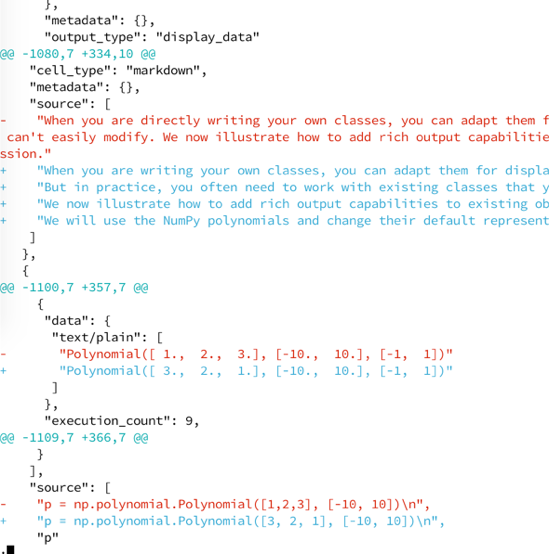
\includegraphics[width=.9\textwidth]{img/json-diff}}
    \caption{Text-based diff of a notebook as JSON, showing additional markup impeding readability.}
    \label{fig:json-diff}
\end{figure}

\begin{figure}
    \center
    \framebox{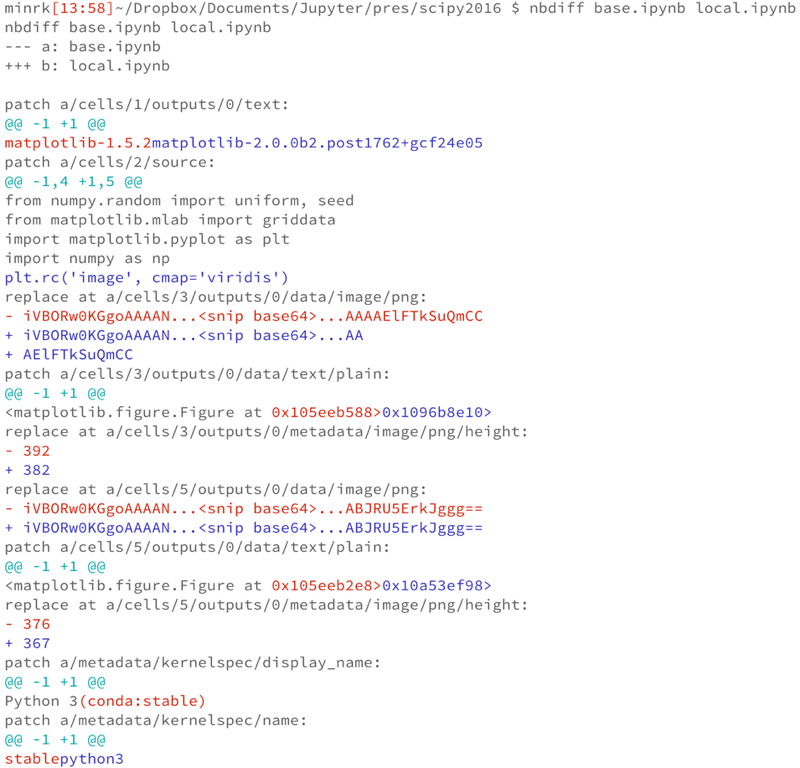
\includegraphics[width=.9\textwidth]{img/nbdiff}}
    \caption{\nbdiff output, including truncated image changes and clearer changes in source code compared to JSON.}
    \label{fig:nbdiff}
\end{figure}

\nbdime provides two mechanisms for comparing notebooks. First is a command-line diff of notebooks
via the \nbdiff command, enabling use in a text-based terminal where developers spend much
of their time. The key for diffing notebooks is that not all information in a notebook has equal
importance, and not all of it is sensibly viewable as text, such as embedded images. The second
important task of \nbdime is displaying text content in a more legible form than the raw JSON. JSON
includes additional structured markup, such as quotation marks, indentation, and escaped
characters, which make the text difficult to read, and appear different from the text a user might
see when they are editing the notebook. By recognizing the structure of the notebook, \nbdime is
able to make intelligent decisions about how to display text without additional markup and deemphasize information that is not viewable in a text-only environment.
\nbdime includes the structure and metadata with minimal markup, designed for humans to read.
When images or other embedded data is seen, it is replaced by an indication that there is binary data that change, rather than the unintelligible difference between the binary data.

\begin{figure}
    \center
    \framebox{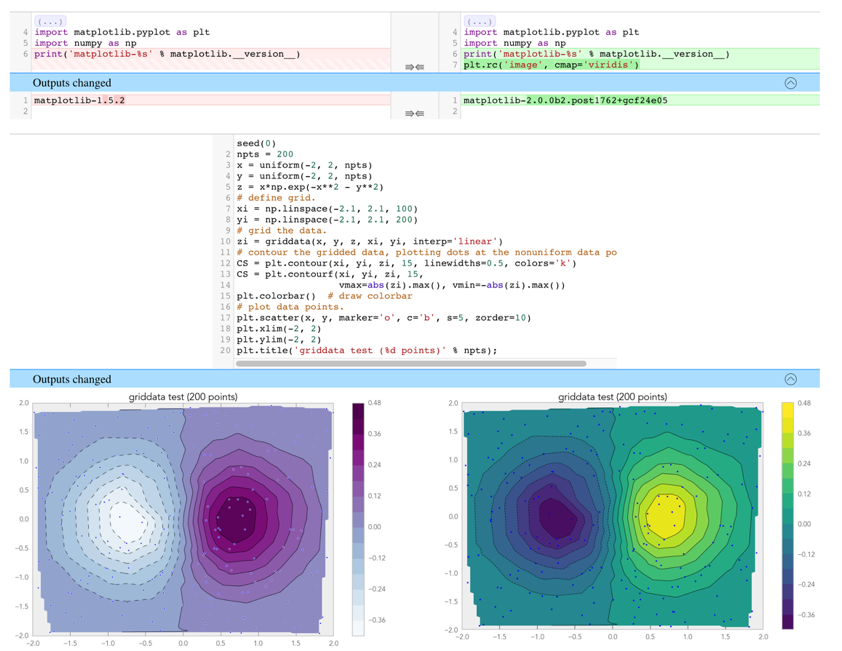
\includegraphics[width=\textwidth]{img/nbdiff-web}}
    \caption{nbdiff-web output showing side-by-side comparison of output images.}
    \label{fig:nbdiff-web}
\end{figure}

\nbdime also provides a web-based diff viewer via the \software{nbdiff-web} command. Notebooks are
most commonly viewed and produced in a web-based environment, with the ability to view rendered
images and HTML. The goal of the web-based viewer is to show the reviewer the actual changes in the
notebook document, including changes in output images and rendered HTML.
This allows the most natural experience of reviewing changes in a document, where the review environment is as similar to the interactive notebook environment as possible.

% section diffing_notebooks (end)

\section{Merging notebooks} % (fold)
\label{sec:merging_notebooks}

\begin{figure}
    \center
    \framebox{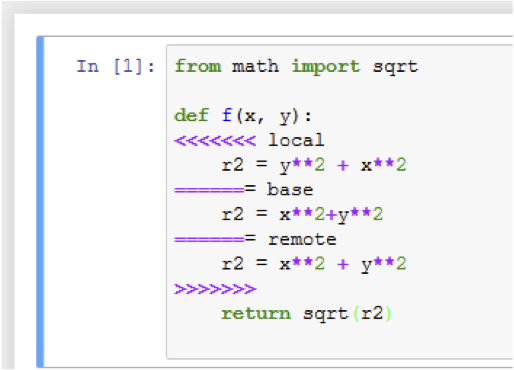
\includegraphics[width=.6\textwidth]{img/nbmerge}}
    \caption{The result of \nbmerge with a conflict is still a valid notebook.}
    \label{fig:nbmerge}
\end{figure}

One challenge for merging two notebooks using text is the structured JSON information, where
text-based merge strategies can result in a syntactically invalid document. This is a problem for
merging all structured documents, including source code in programming languages such as C, Python,
or \LaTeX. However, for tools where the editor is not plain-text, such as notebooks, preventing the
creation of these invalid documents is particularly important. Another challenge for merging is the
fact that some of the content in notebooks is generated, and thus should be treated differently
when considering conflicts between two change sets.

\nbdime addresses the issue of conflicts with its own merge mechanism, always ensuring that a valid notebook is the result, even if there are conflicts.
The second task of \nbdime's merge tool is to allow users to ignore conflicts on certain fields of the notebook.
There is a hierarchy of significance in the content of notebooks,
and not all changes should be considered conflicting.
For instance, if two change sets both alter certain metadata,
the changes are not significant and automatic resolution of conflicts
can be carried out aggressively by clearing conflicting values.
Similarly for generated output, conflicts can be automatically resolved without the consequences of automatic resolution in the source code.
It remains possible to be strict about differences in output,
especially as it pertains to evaluating the reproducibility of notebooks.
In the worst case scenario, a notebook can be re-executed to produce new output.


\begin{figure}
    \center
    \framebox{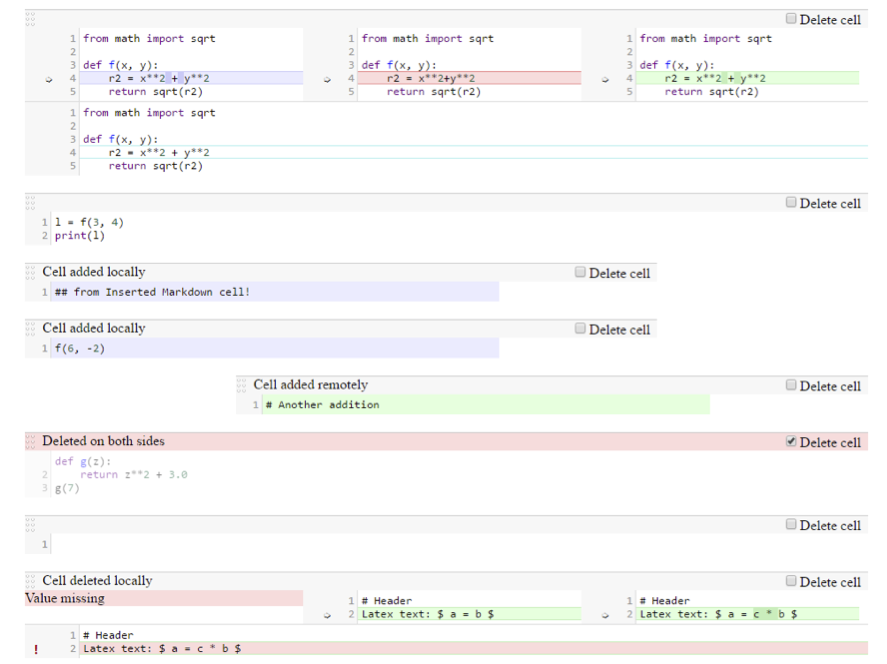
\includegraphics[width=\textwidth]{img/nbmerge-web}}
    \caption{\nbmerge web-based merge conflict resolution tool allows individual conflict resolution.}
    \label{fig:nbmerge-web}
\end{figure}

When merge conflicts do occur, the \nbmerge web tool can be used to view and resolve the conflicting changes one by one.

% section merging_notebooks (end)


\section{Version control integration} % (fold)
\label{sub:version_control_integration}

\nbdime provides integration with the git version control system for its diffing and merging tools.
Git provides two mechanisms for integrating external software for
performing the diff and merge operations on specific files.

The first is called a "driver", and is used internally by git when computing diffs and performing merges. \nbdime can register its command-line diff rendering as a diff driver for notebook files.
This can be done as a system-wide configuration, or for individual git repositories.
\nbdime also provides a merge driver for auto-resolving conflicts on notebooks,
ensuring that a \software{git merge} never results in an invalid notebook document,
and that conflicts can be resolved in the user's familiar notebook-editing environment.

The second git integration point is called a "tool", e.g. "difftool" or "mergetool".
These are like drivers, but allow external applications that may open windows to be launched.
\nbdime provides tool entrypoints for diff and merge to launch the web interfaces for viewing diffs
and manually resolving merge conflicts.

% subsection version_control_integration (end)

\section{\nbdime and reproducibility} % (fold)
\label{sec:nbdime_and_reproducibility}

Efficiently comparing notebooks and their output benefits the goals of OpenDreamKit,
especially as it improves the ability of scientists and developers to follow reproducible workflows.
By better integrating with version control systems,
best practices in reproducibility are encouraged and facilitated,
and verification of changes in notebooks is enabled.
Further work in \delivref{UI}{jupyter-test} (Facilities for running notebooks as verification tests)
can leverage \nbdime to trace and identify changes in notebooks,
leading to verification tools that can efficiently evaluate the reproducibility of notebooks.

% section nbdime_and_reproducibility (end)
\section{Future work}

The current version of \nbdime is a working prototype but we expect
some more work to be necessary to make it a polished product.
Designers from the wider \Jupyter community will be involved in
polishing the visual presentation of the web interfaces,
and users will become involved in further testing once the tool
reaches a wider user base. Furthermore we expect to be able to
improve the algorithms used for diffing and merging further,
both for improving the diff quality and performance.

While \nbdime integrates well into the local git workflow of diffing
and merging, much of the diffing and merging work of today's
scientists and developers happens on public websites such as GitHub or
Bitbucket, where the user cannot customize the diffing or merging
behavior.  However, these websites do support custom diff viewing of
certain file types, such as images and GeoJSON files.  After some
maturation of the design of the \software{nbdime-web diff} viewer, we
will work with GitHub and others to integrate diff viewing of
notebooks into their websites, as we have done in the past with
rendering of single notebooks.  By integrating \nbdime with remote
notebook editing tools like \software{JupyterLab}, comparing notebooks
on remote servers should become much easier than today, and would
integrate well with such a development process.

\end{document}

